\chapter{Conclusion}

\todo{first finish the whole thesis, then the intro and then come back to rewrite the first sentence}
We got almost $4$ orders of magnitude improvement in the relative error both in the \ac{UWF}\index{UWF}($n=64$, $m=640$, 
and in the unfolded $L=160$ times) and the \ac{URWF}\index{URWF}($n=64$, $m=640$, and unfolded $L=30$ times) after performing 
\ho \cite{Hutter2019}\cite{Akiba2019}\index{\hp} compared to the \ac{WF}\cite{Candes2014}\index{\ac{WF}} 
\cref{pseudocode:wf} and the \ac{RWF}\cite{Zhang2016}\index{\ac{RWF}} 
\cref{pseudocode:rwf} using the same number of iteration which can be seen in 
\cref{fig:proposed_winning_scenarios} which is a smaller sized version of \cref{fig:uwf_training_07_08_optuna} and 
in \cref{fig:proposed_winning_scenarios} which is a smaller sized version of \cref{fig:urwf_training_07_08_optuna}. The model is still 
interpretable thanks to the scenarios we considered as we were only focusing on tinkering with the step size and therefore 
the total structure of the iterative algorithm is intact(We did not change the innate nonlinearities associated with the algorithms). 
The datasets are very small(only $100$ samples) compared to today's \ml/\dl \cite{Goodfellow2016}\cite{LeCun2015} 
counterparts' \cite{Krizhevsky2017}\cite{Szegedy2014} datasets(millions of samples). Increasing the the number of samples from $100$ to $500$ resulted in almost 
no improvement in the relative error. In the proposed winning scenarios, different scalars multiplied by a single matrix of the form $\tau_k\boldsymbol{M}$, you only need to train 
$n^2+L$(around $4100$ for both the \ac{UWF} and the \ac{URWF}) parameters which tremendously reduces the required number of 
\ac{FLOPS}\cite{Hager2010}\cite{Hennessy2019}\index{\ac{FLOPS}} and in turn training time to reach satisfactory 
relative errors both on the train and the test data. If we were to use a fully connected multi-perceptron \nn we would have 
had, depending on the exact architecture, roughly $Lmn$(around $1.2$ million for the \ac{URWF} and around $6.5$ million for the \ac{UWF}) 
As another example to show the sheer size of the general contemporary \ml/\dl models and put that into perspective, 
ImageNet\cite{Deng2009}\index{ImageNet} has around $14$ millions images and a relatively new model like GoogleNet\cite{Szegedy2014}\index{GoogleNet}, 
depending on the instance that you use, has millions of parameters only to classify an image as one of the $1000$ 
classes. What got me very interested in taking \du/\au\cite{Monga2019} as my thesis topic was to go for \ml/\dl models with relatively few number of parameters 
rather than the general direction that is currently trending. If you are reading this, it is my hope that my work could 
somehow win you over and convince you that small does not always mean weak.


% \afterpage{%
%   \clearpage % Start a new page
\begin{figure}[!htbp]
    \captionsetup{justification=centering}
%   \subfloat[Different Matrices$(\boldsymbol{M}_k)$, $\mathrm{lr}=1.000\times10^{-3}, \,\mathrm{L}=30$]{% This file was created with tikzplotlib v0.10.1.
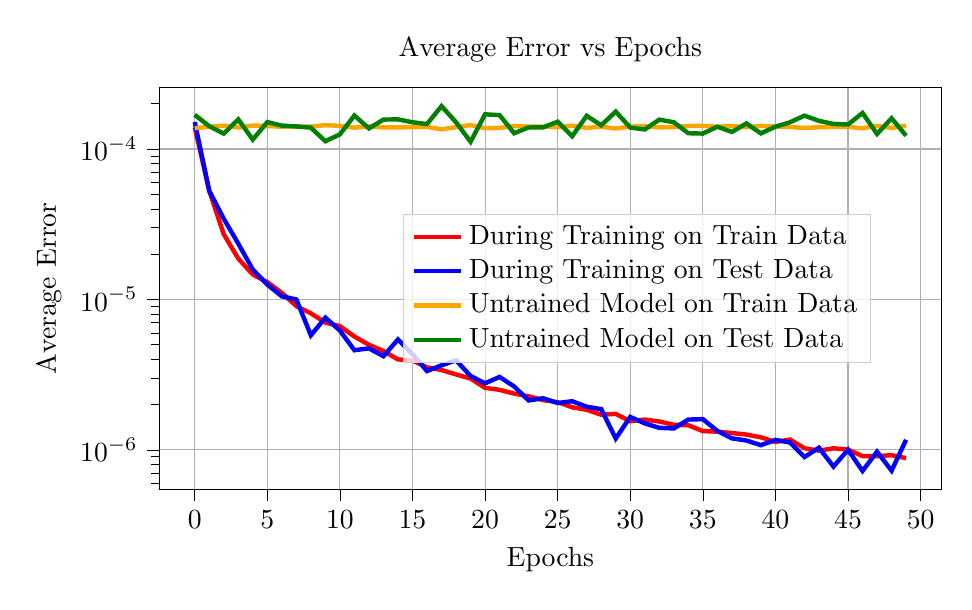
\begin{tikzpicture}

  \definecolor{darkgray176}{RGB}{176,176,176}
  \definecolor{green}{RGB}{0,128,0}
  \definecolor{lightgray204}{RGB}{204,204,204}
  \definecolor{orange}{RGB}{255,165,0}
  
  \begin{axis}[
    width = 0.95\textwidth,
    height = 19em,
  legend cell align={left},
  legend style={
    fill opacity=0.8,
    draw opacity=1,
    text opacity=1,
    at={(0.91,0.5)},
    anchor=east,
    draw=lightgray204
  },
  % log basis y={10},
  tick align=outside,
  tick pos=left,
  title={Average Error vs Epochs},
  x grid style={darkgray176},
  xlabel={Epochs},
  xmajorgrids,
  xmin=-2.45, xmax=51.45,
  xtick style={color=black},
  y grid style={darkgray176},
  ylabel={Average Error},
  ymajorgrids,
  ymin=5.47956319196448e-07, ymax=0.000254691381547786,
  ymode=log,
  ytick style={color=black},
  ytick={1e-08,1e-07,1e-06,1e-05,0.0001,0.001,0.01},
  yticklabels={
    \(\displaystyle {10^{-8}}\),
    \(\displaystyle {10^{-7}}\),
    \(\displaystyle {10^{-6}}\),
    \(\displaystyle {10^{-5}}\),
    \(\displaystyle {10^{-4}}\),
    \(\displaystyle {10^{-3}}\),
    \(\displaystyle {10^{-2}}\)
  }
  ]
  \addplot [ultra thick, red]
table {%
0 0.000139422554639168
1 5.25441355421208e-05
2 2.709246109589e-05
3 1.86883116839454e-05
4 1.4641495909018e-05
5 1.30382604766055e-05
6 1.10479877548642e-05
7 9.03117143025156e-06
8 8.08377171779284e-06
9 7.014934453764e-06
10 6.64117942505982e-06
11 5.66791140954592e-06
12 4.99323004987673e-06
13 4.53997472504852e-06
14 3.99270811612951e-06
15 3.92411902794265e-06
16 3.53491191162902e-06
17 3.39455823450407e-06
18 3.1713191219751e-06
19 2.97965834761271e-06
20 2.58465047409118e-06
21 2.5051617740246e-06
22 2.36605910686194e-06
23 2.27213763537293e-06
24 2.14105693885358e-06
25 2.07581410904822e-06
26 1.91861840903584e-06
27 1.84637030997692e-06
28 1.71315411989781e-06
29 1.73497676314582e-06
30 1.54966937770951e-06
31 1.59103592523024e-06
32 1.54397719143162e-06
33 1.46790443977807e-06
34 1.45789761063497e-06
35 1.33272737912193e-06
36 1.32122954710212e-06
37 1.2942375633429e-06
38 1.26361408092635e-06
39 1.21193875202152e-06
40 1.12860448098218e-06
41 1.17169065561029e-06
42 1.0251166031594e-06
43 9.8811494808615e-07
44 1.02411047464557e-06
45 1.00423574167507e-06
46 9.08802235244366e-07
47 9.08564288693015e-07
48 9.21839614420605e-07
49 8.81109031070082e-07
};
\addlegendentry{During Training on Train Data}
\addplot [ultra thick, blue]
table {%
0 0.000151191532495432
1 5.27330812474247e-05
2 3.43467727361713e-05
3 2.34825092775282e-05
4 1.57967224367894e-05
5 1.25444585137302e-05
6 1.04895107142511e-05
7 9.99405347101856e-06
8 5.77313267058344e-06
9 7.56428335080273e-06
10 6.20858509137179e-06
11 4.59601551483502e-06
12 4.72754800284747e-06
13 4.19237494497793e-06
14 5.41578947377275e-06
15 4.31831585956388e-06
16 3.34092874254566e-06
17 3.64814991371532e-06
18 3.93835989598301e-06
19 3.09812821797095e-06
20 2.76999890047591e-06
21 3.05379262499628e-06
22 2.63992797044921e-06
23 2.13079511013348e-06
24 2.2038937004254e-06
25 2.0483175831032e-06
26 2.10558482649503e-06
27 1.93491723621264e-06
28 1.86590375506057e-06
29 1.18982120511646e-06
30 1.65560504683526e-06
31 1.49886989220249e-06
32 1.40136648951739e-06
33 1.38726443310588e-06
34 1.5903664234429e-06
35 1.600476934982e-06
36 1.33635251131636e-06
37 1.19272579013341e-06
38 1.15448892756831e-06
39 1.07466962617764e-06
40 1.16404714844975e-06
41 1.11877704966901e-06
42 8.96443566489324e-07
43 1.03346019386663e-06
44 7.74358625221794e-07
45 1.00108979950164e-06
46 7.24411620467436e-07
47 9.72342604654841e-07
48 7.2755648261591e-07
49 1.16638921099366e-06
};
\addlegendentry{During Training on Test Data}
\addplot [ultra thick, orange]
table {%
0 0.000137548107886687
1 0.000140638832817785
2 0.000142808101372793
3 0.000138855073601007
4 0.00014315867156256
5 0.000142147371661849
6 0.000140535441460088
7 0.000140832271426916
8 0.000141012889798731
9 0.000143917815876193
10 0.000142426055390388
11 0.000138538351166062
12 0.000141437121783383
13 0.000139053459861316
14 0.000139040130306967
15 0.000139728872454725
16 0.000140273332362995
17 0.00013496758765541
18 0.000139760843012482
19 0.000144059871672653
20 0.000137425566208549
21 0.000137912458740175
22 0.000142265387694351
23 0.000140677715535276
24 0.000141052427352406
25 0.000139516676426865
26 0.00014278301387094
27 0.000138091811095364
28 0.000140507239848375
29 0.000136786737130024
30 0.00014075510262046
31 0.000142040196806192
32 0.000139078518259339
33 0.000139772397233173
34 0.000142270961077884
35 0.000142297969432548
36 0.000140746793476865
37 0.000141959739266895
38 0.000139722877065651
39 0.000142463482916355
40 0.000140872885822318
41 0.00014001976524014
42 0.000137886876473203
43 0.000139517200295813
44 0.00014015486522112
45 0.000140228410600685
46 0.000137308554258198
47 0.00014238734729588
48 0.000138002840685658
49 0.000142704491736367
};
\addlegendentry{Untrained Model on Train Data}
\addplot [ultra thick, green]
table {%
0 0.000168594866408966
1 0.000141678872751072
2 0.000126560087664984
3 0.000157214250066318
4 0.000115438073407859
5 0.000150999199831858
6 0.000142947799758986
7 0.000141304670250975
8 0.000138527931994759
9 0.000112627378257457
10 0.000125072823720984
11 0.000166890022228472
12 0.000136944450787269
13 0.000156815774971619
14 0.000157319751451723
15 0.000150483218021691
16 0.000146467093145475
17 0.00019265255832579
18 0.000150442734593526
19 0.000111669789475854
20 0.000169916238519363
21 0.000167860955116339
22 0.000127240127767436
23 0.000138955030706711
24 0.000139115072670393
25 0.000151672968058847
26 0.000121595592645463
27 0.000166218713275157
28 0.000143689205287956
29 0.000177146794158034
30 0.000138729737955146
31 0.000134799440274946
32 0.00015673965390306
33 0.000150496722199023
34 0.000127258579595946
35 0.000126562154036947
36 0.000140600168379024
37 0.000129729727632366
38 0.000147858329000883
39 0.000126872822875157
40 0.000140709613333456
41 0.000150389416376129
42 0.000166537720360793
43 0.000153616216266528
44 0.000146757418406196
45 0.000145377474837005
46 0.000173495995113626
47 0.000125866179587319
48 0.000159938761498779
49 0.000122543351608329
};
\addlegendentry{Untrained Model on Test Data}
\end{axis}

\end{tikzpicture}}\\  
%   \subfloat[Different Semi-Positive Definite Matrices$(\boldsymbol{S}_k)$, $\mathrm{lr}=1.000\times10^{-3}, \,\mathrm{L}=30$]{% This file was created with tikzplotlib v0.10.1.
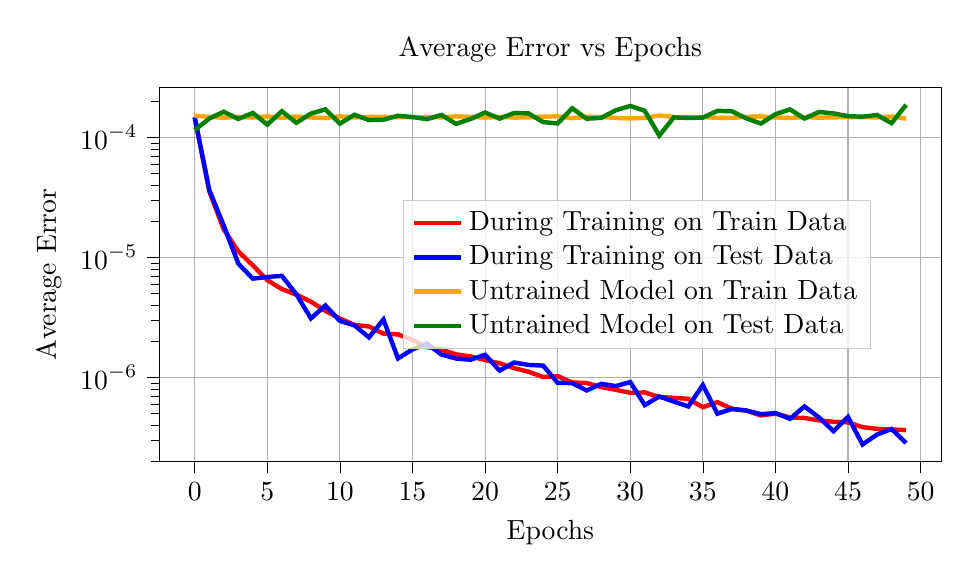
\begin{tikzpicture}

  \definecolor{darkgray176}{RGB}{176,176,176}
  \definecolor{green}{RGB}{0,128,0}
  \definecolor{lightgray204}{RGB}{204,204,204}
  \definecolor{orange}{RGB}{255,165,0}
  
  \begin{axis}[
    width = 0.95\textwidth,
    height = 18em,
  legend cell align={left},
  legend style={
    fill opacity=0.8,
    draw opacity=1,
    text opacity=1,
    at={(0.91,0.5)},
    anchor=east,
    draw=lightgray204
  },
  % log basis y={10},
  tick align=outside,
  tick pos=left,
  title={Average Error vs Epochs},
  x grid style={darkgray176},
  xlabel={Epochs},
  xmajorgrids,
  xmin=-2.45, xmax=51.45,
  xtick style={color=black},
  y grid style={darkgray176},
  ylabel={Average Error},
  ymajorgrids,
  ymin=1.98989848731464e-07, ymax=0.00025862395496495,
  ymode=log,
  ytick style={color=black},
  ytick={1e-08,1e-07,1e-06,1e-05,0.0001,0.001,0.01},
  yticklabels={
    \(\displaystyle {10^{-8}}\),
    \(\displaystyle {10^{-7}}\),
    \(\displaystyle {10^{-6}}\),
    \(\displaystyle {10^{-5}}\),
    \(\displaystyle {10^{-4}}\),
    \(\displaystyle {10^{-3}}\),
    \(\displaystyle {10^{-2}}\)
  }
  ]
  \addplot [ultra thick, red]
  table {%
  0 0.000148013044963591
  1 3.56593227479607e-05
  2 1.7092230336857e-05
  3 1.12235911728931e-05
  4 8.58035764395026e-06
  5 6.45710269964184e-06
  6 5.44462363905041e-06
  7 4.88857358504902e-06
  8 4.2726201172627e-06
  9 3.58169586434087e-06
  10 3.09524739350309e-06
  11 2.73389900939947e-06
  12 2.65521657638601e-06
  13 2.31281637752545e-06
  14 2.27968439503456e-06
  15 2.05286619348044e-06
  16 1.78653704097087e-06
  17 1.69934662608284e-06
  18 1.55517341227096e-06
  19 1.49384698033828e-06
  20 1.3938711163064e-06
  21 1.30992964386678e-06
  22 1.19467654258187e-06
  23 1.11279143766296e-06
  24 1.00586737517006e-06
  25 1.02330841400544e-06
  26 9.0733004753929e-07
  27 8.96316521448171e-07
  28 8.29465079732472e-07
  29 7.87274132107996e-07
  30 7.43528971725027e-07
  31 7.48820809803874e-07
  32 6.85715860981873e-07
  33 6.74960119795287e-07
  34 6.62006982565799e-07
  35 5.64021263471659e-07
  36 6.21000424416707e-07
  37 5.4747005151512e-07
  38 5.2761015467695e-07
  39 4.81172207855707e-07
  40 4.98232964218914e-07
  41 4.6397821051869e-07
  42 4.58541705938842e-07
  43 4.38037005778824e-07
  44 4.26196010039348e-07
  45 4.2150298895649e-07
  46 3.84383071150296e-07
  47 3.72081899513432e-07
  48 3.67385837307665e-07
  49 3.63334208941524e-07
  };
  \addlegendentry{During Training on Train Data}
  \addplot [ultra thick, blue]
  table {%
  0 0.000145961690577678
  1 3.6507273762254e-05
  2 1.83924421435222e-05
  3 8.87434453034075e-06
  4 6.65402694721706e-06
  5 6.85723716742359e-06
  6 7.01677663528244e-06
  7 4.92142953589791e-06
  8 3.10200198327948e-06
  9 3.96965651816572e-06
  10 2.95227073365822e-06
  11 2.71325984613213e-06
  12 2.15284285332018e-06
  13 3.03261163026036e-06
  14 1.43896522786235e-06
  15 1.70873647675762e-06
  16 1.90969149116427e-06
  17 1.54746635416814e-06
  18 1.43470697366865e-06
  19 1.4017372222952e-06
  20 1.54278404806973e-06
  21 1.13814337510121e-06
  22 1.32910520278529e-06
  23 1.26849226944614e-06
  24 1.25276187645795e-06
  25 9.00273789739003e-07
  26 8.95020548341563e-07
  27 7.7743254678353e-07
  28 8.83171367149771e-07
  29 8.45460078835458e-07
  30 9.13137625957461e-07
  31 5.87568308674236e-07
  32 6.92485286890587e-07
  33 6.28680254521896e-07
  34 5.71698194562487e-07
  35 8.63643435877748e-07
  36 4.98133147175395e-07
  37 5.44820807135693e-07
  38 5.29007309069129e-07
  39 4.93094887588086e-07
  40 5.04310378346418e-07
  41 4.50991336720108e-07
  42 5.72123838082916e-07
  43 4.63405569917086e-07
  44 3.56029943304748e-07
  45 4.6835725697747e-07
  46 2.75656987014372e-07
  47 3.33770287852531e-07
  48 3.71070939308993e-07
  49 2.83416682123061e-07
  };
  \addlegendentry{During Training on Test Data}
  \addplot [ultra thick, orange]
  table {%
  0 0.000151286862092093
  1 0.000148271938087419
  2 0.000145962316310033
  3 0.000148140708915889
  4 0.000146270336699672
  5 0.000149768020492047
  6 0.000145538549986668
  7 0.000149274768773466
  8 0.000146568301715888
  9 0.000144949066452682
  10 0.00014968030154705
  11 0.000146915088407695
  12 0.000148198654642329
  13 0.000148643390275538
  14 0.000147157494211569
  15 0.000147706436109729
  16 0.00014777151227463
  17 0.00014694788842462
  18 0.000149669518577866
  19 0.000148425155202858
  20 0.000146184596815147
  21 0.000148376799188554
  22 0.000146324280649424
  23 0.00014655634004157
  24 0.000149089726619422
  25 0.000149657396832481
  26 0.000144709527376108
  27 0.000148061357322149
  28 0.000147991930134594
  29 0.000145307276397943
  30 0.000143848243169487
  31 0.000145373909617774
  32 0.000152415770571679
  33 0.000147752347402275
  34 0.00014776736497879
  35 0.000147837854456156
  36 0.000145569443702698
  37 0.000145633559441194
  38 0.000148161940160207
  39 0.000149608822539449
  40 0.000146714635775425
  41 0.000145101090311073
  42 0.000147954560816288
  43 0.000146047284943052
  44 0.000147063998156227
  45 0.000147197628393769
  46 0.000147608181578107
  47 0.000146761129144579
  48 0.000149398503708653
  49 0.000143366807606071
  };
  \addlegendentry{Untrained Model on Train Data}
  \addplot [ultra thick, green]
  table {%
  0 0.000115061491669621
  1 0.000143547338666394
  2 0.000163512173458003
  3 0.000142517077620141
  4 0.000159814182552509
  5 0.00012783041165676
  6 0.000165362667758018
  7 0.000132426110212691
  8 0.000157876085722819
  9 0.000171300649526529
  10 0.000130172455101274
  11 0.000154473222210072
  12 0.000139474926982075
  13 0.000140412186738104
  14 0.000151597065269016
  15 0.00014767273387406
  16 0.000141933254781179
  17 0.000153813511133194
  18 0.000129606123664416
  19 0.000142261982546188
  20 0.000161294257850386
  21 0.00014334442676045
  22 0.000159681003424339
  23 0.000158348615514114
  24 0.000134108049678616
  25 0.000130705229821615
  26 0.000174892600625753
  27 0.000143100725836121
  28 0.000145519719808362
  29 0.000168184196809307
  30 0.000182958712684922
  31 0.000166574260219932
  32 0.000103557540569454
  33 0.000146681413752958
  34 0.000145311874803156
  35 0.00014605671458412
  36 0.000166460915352218
  37 0.000165033299708739
  38 0.000144075253047049
  39 0.000130360465846024
  40 0.000155840680235997
  41 0.000171156978467479
  42 0.000143605619086884
  43 0.000162815587827936
  44 0.000158585360622965
  45 0.000150236810441129
  46 0.000148762876051478
  47 0.000153807501192205
  48 0.000131454333313741
  49 0.000186694131116383
  };
  \addlegendentry{Untrained Model on Test Data}
  \end{axis}
  
  \end{tikzpicture}
  }\\  
\resizebox{1.0\textwidth}{!}{
  \subfloat[Proposed Winning Scenario for \ac{UWF} Using \optuna\cite{Akiba2019}\index{\optuna}: Different Scalars Multiplied by a Single Matrix$(\tau_k\boldsymbol{M})$, $\mathrm{lr}=8.798\times10^{-3}, \,\mathrm{L}=160$]{% This file was created with tikzplotlib v0.10.1.
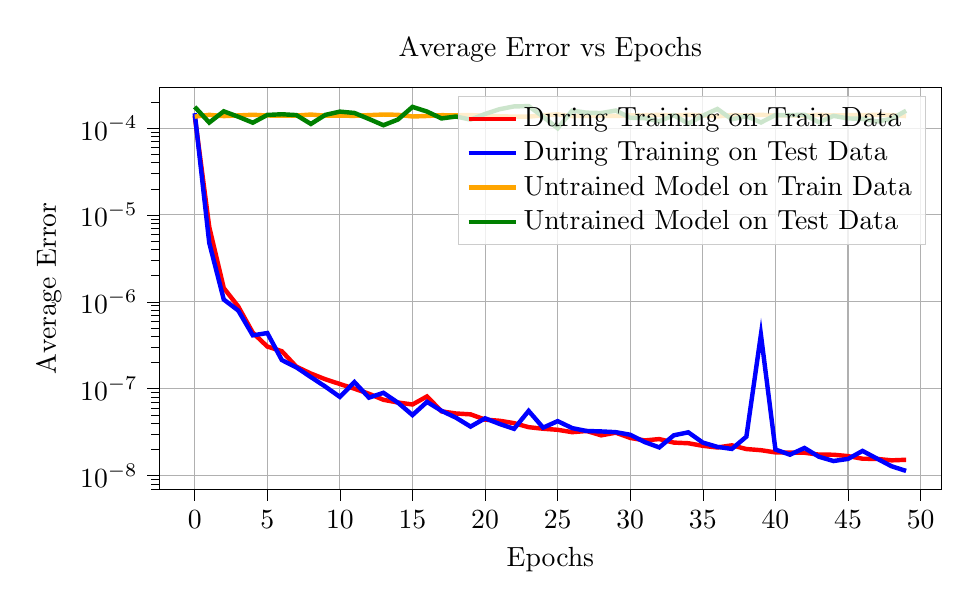
\begin{tikzpicture}

    \definecolor{darkgray176}{RGB}{176,176,176}
    \definecolor{green}{RGB}{0,128,0}
    \definecolor{lightgray204}{RGB}{204,204,204}
    \definecolor{orange}{RGB}{255,165,0}
    
    \begin{axis}[
        width = 0.95\textwidth,
        height = 19em,
    legend cell align={left},
    legend style={
      fill opacity=0.8,
      draw opacity=1,
      text opacity=1,
    %   at={(0.5,0.5)},
    %   anchor=center,
      draw=lightgray204
    },
    % log basis y={10},
    tick align=outside,
    tick pos=left,
    title={Average Error vs Epochs},
    x grid style={darkgray176},
    xlabel={Epochs},
    xmajorgrids,
    xmin=-2.45, xmax=51.45,
    xtick style={color=black},
    y grid style={darkgray176},
    ylabel={Average Error},
    ymajorgrids,
    ymin=6.96321187378274e-09, ymax=0.000290354904410608,
    ymode=log,
    ytick style={color=black},
    ytick={1e-10,1e-09,1e-08,1e-07,1e-06,1e-05,0.0001,0.001,0.01},
    yticklabels={
      \(\displaystyle {10^{-10}}\),
      \(\displaystyle {10^{-9}}\),
      \(\displaystyle {10^{-8}}\),
      \(\displaystyle {10^{-7}}\),
      \(\displaystyle {10^{-6}}\),
      \(\displaystyle {10^{-5}}\),
      \(\displaystyle {10^{-4}}\),
      \(\displaystyle {10^{-3}}\),
      \(\displaystyle {10^{-2}}\)
    }
    ]
    \addplot [ultra thick, red]
    table {%
    0 0.000138899733428843
    1 7.26432836017921e-06
    2 1.44128989632009e-06
    3 8.82225094755995e-07
    4 4.4099317619839e-07
    5 3.05433417224776e-07
    6 2.6985495082954e-07
    7 1.79246782749942e-07
    8 1.49264380411296e-07
    9 1.28192979786945e-07
    10 1.13041885185794e-07
    11 9.98787328398976e-08
    12 8.73495338282737e-08
    13 7.44121209095283e-08
    14 6.92524650958148e-08
    15 6.57125269754033e-08
    16 8.13764842177989e-08
    17 5.47648397741796e-08
    18 5.17549807454998e-08
    19 5.06033721592303e-08
    20 4.39799201501501e-08
    21 4.26815560672367e-08
    22 4.00799038402511e-08
    23 3.60131551246923e-08
    24 3.45376491850402e-08
    25 3.35878418411539e-08
    26 3.15419796947936e-08
    27 3.25466764650173e-08
    28 2.90125079516201e-08
    29 3.11344905412625e-08
    30 2.70826809867231e-08
    31 2.53443790398933e-08
    32 2.6274593167841e-08
    33 2.39348345587587e-08
    34 2.35225705580433e-08
    35 2.19639648690872e-08
    36 2.10294555103019e-08
    37 2.22524789705858e-08
    38 2.01735375071621e-08
    39 1.95676985725868e-08
    40 1.84541022463236e-08
    41 1.83214634574824e-08
    42 1.82840071971668e-08
    43 1.73900591704523e-08
    44 1.73470766640094e-08
    45 1.67271281270587e-08
    46 1.56075810053835e-08
    47 1.55275490243412e-08
    48 1.49438257324164e-08
    49 1.51756438526718e-08
    };
    \addlegendentry{During Training on Train Data}
    \addplot [ultra thick, blue]
    table {%
    0 0.00014844533870928
    1 4.76674267702037e-06
    2 1.0628197060214e-06
    3 7.92268110672012e-07
    4 4.11031038538567e-07
    5 4.36832323202907e-07
    6 2.13414253380506e-07
    7 1.75729226725707e-07
    8 1.35837808556971e-07
    9 1.0546255424515e-07
    10 8.0311629346852e-08
    11 1.19002564247239e-07
    12 7.88221186098781e-08
    13 8.94856313493619e-08
    14 6.89524028985034e-08
    15 4.96274097372407e-08
    16 7.04482232549708e-08
    17 5.55252590572763e-08
    18 4.62508005227846e-08
    19 3.654967173361e-08
    20 4.55651267827761e-08
    21 3.92327486054e-08
    22 3.44960220388657e-08
    23 5.54300179089751e-08
    24 3.55577576272026e-08
    25 4.22732249205637e-08
    26 3.51410207599656e-08
    27 3.25441220638822e-08
    28 3.21748352405393e-08
    29 3.15483639212744e-08
    30 2.94743696116484e-08
    31 2.42509656800394e-08
    32 2.1060678534468e-08
    33 2.90387500712086e-08
    34 3.14091828101937e-08
    35 2.39285675718293e-08
    36 2.13697148865322e-08
    37 2.02332923748827e-08
    38 2.80337761893179e-08
    39 4.1882645973601e-07
    40 1.9922834937347e-08
    41 1.73602039410525e-08
    42 2.07416608333233e-08
    43 1.64387952139577e-08
    44 1.46818992519115e-08
    45 1.55218575770277e-08
    46 1.92011722077723e-08
    47 1.56486414937262e-08
    48 1.27744943512198e-08
    49 1.12931486384582e-08
    };
    \addlegendentry{During Training on Test Data}
    \addplot [ultra thick, orange]
    table {%
    0 0.000135580819915049
    1 0.000142116216011345
    2 0.000137380717205815
    3 0.000139936193590984
    4 0.000142444492666982
    5 0.000139559400849976
    6 0.000139205061714165
    7 0.000139498966746032
    8 0.000143201788887382
    9 0.000139012030558661
    10 0.000138873860123567
    11 0.000138410890940577
    12 0.00014102082059253
    13 0.000143270721309818
    14 0.000142237113323063
    15 0.000135978290927596
    16 0.000137778275529854
    17 0.00014073250349611
    18 0.000140512682264671
    19 0.000141123935463838
    20 0.00013889440742787
    21 0.000137015958898701
    22 0.00013543690147344
    23 0.000135413778480142
    24 0.000140565694891848
    25 0.000144005738548003
    26 0.000137403549160808
    27 0.00013848849630449
    28 0.000138961564516649
    29 0.00013785291230306
    30 0.000140357617055997
    31 0.000140674586873502
    32 0.000142057760967873
    33 0.000139720403240062
    34 0.000142506891279481
    35 0.000140076066600159
    36 0.000136208720505238
    37 0.000141315162181854
    38 0.000139822936034761
    39 0.000142146338475868
    40 0.000139813200803474
    41 0.000139538722578436
    42 0.000139243988087401
    43 0.000142359247547574
    44 0.000139776835567318
    45 0.000140800751978531
    46 0.000140809308504686
    47 0.000142282297019847
    48 0.000141126482049003
    49 0.000137355818878859
    };
    \addlegendentry{Untrained Model on Train Data}
    \addplot [ultra thick, green]
    table {%
    0 0.000175602370291017
    1 0.000115721581096295
    2 0.000156029564095661
    3 0.000135122318170033
    4 0.000115373361040838
    5 0.000141736381920055
    6 0.000144295612699352
    7 0.000141208045533858
    8 0.000111631678009871
    9 0.000142020973726176
    10 0.000154777924763039
    11 0.000149349492858164
    12 0.000127313614939339
    13 0.000107892628875561
    14 0.000125519931316376
    15 0.000175431167008355
    16 0.000155052868649364
    17 0.00012920267181471
    18 0.000135864058393054
    19 0.000125273712910712
    20 0.000145317215356044
    21 0.000164944241987541
    22 0.000177754482137971
    23 0.000179029142600484
    24 0.000135274472995661
    25 9.9544799013529e-05
    26 0.000158733208081685
    27 0.000150573701830581
    28 0.000148892766446806
    29 0.000159243267262354
    30 0.000131555570987985
    31 0.000129963023937307
    32 0.00011968205217272
    33 0.000140874632052146
    34 0.000112492547486909
    35 0.000139083160320297
    36 0.0001660277339397
    37 0.000126232087495737
    38 0.000137334165628999
    39 0.000116096263809595
    40 0.000141106240334921
    41 0.000140998396091163
    42 0.000142489516292699
    43 0.000116595139843412
    44 0.000138309842441231
    45 0.000129201245727018
    46 0.000127760227769613
    47 0.000119176627777051
    48 0.00012781129044015
    49 0.000158458482474089
    };
    \addlegendentry{Untrained Model on Test Data}
    \end{axis}
    
    \end{tikzpicture}
    }\\  
% }
% \resizebox{0.67\textwidth}{!}{
  \subfloat[Proposed Winning Scenario for \ac{URWF} Using \optuna\cite{Akiba2019}\index{\optuna}: Different Scalars Multiplied by a Single Matrix$(\tau_k\boldsymbol{M})$, $\mathrm{lr}=7.622\times10^{-3}, \,\mathrm{L}=30$]{% This file was created with tikzplotlib v0.10.1.
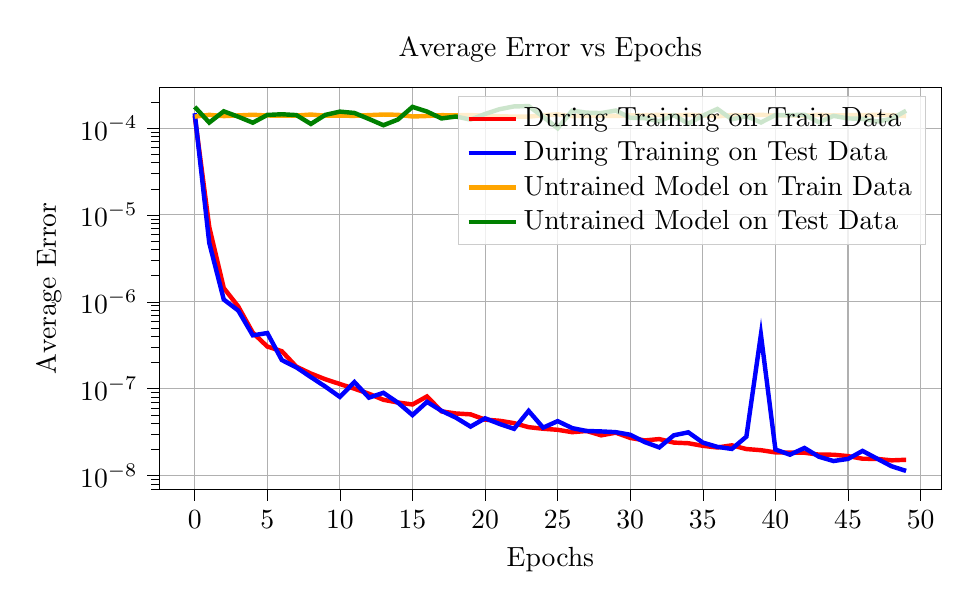
\begin{tikzpicture}

    \definecolor{darkgray176}{RGB}{176,176,176}
    \definecolor{green}{RGB}{0,128,0}
    \definecolor{lightgray204}{RGB}{204,204,204}
    \definecolor{orange}{RGB}{255,165,0}
    
    \begin{axis}[
        width = 0.95\textwidth,
        height = 19em,
    legend cell align={left},
    legend style={
      fill opacity=0.8,
      draw opacity=1,
      text opacity=1,
    %   at={(0.5,0.5)},
    %   anchor=center,
      draw=lightgray204
    },
    % log basis y={10},
    tick align=outside,
    tick pos=left,
    title={Average Error vs Epochs},
    x grid style={darkgray176},
    xlabel={Epochs},
    xmajorgrids,
    xmin=-2.45, xmax=51.45,
    xtick style={color=black},
    y grid style={darkgray176},
    ylabel={Average Error},
    ymajorgrids,
    ymin=6.96321187378274e-09, ymax=0.000290354904410608,
    ymode=log,
    ytick style={color=black},
    ytick={1e-10,1e-09,1e-08,1e-07,1e-06,1e-05,0.0001,0.001,0.01},
    yticklabels={
      \(\displaystyle {10^{-10}}\),
      \(\displaystyle {10^{-9}}\),
      \(\displaystyle {10^{-8}}\),
      \(\displaystyle {10^{-7}}\),
      \(\displaystyle {10^{-6}}\),
      \(\displaystyle {10^{-5}}\),
      \(\displaystyle {10^{-4}}\),
      \(\displaystyle {10^{-3}}\),
      \(\displaystyle {10^{-2}}\)
    }
    ]
    \addplot [ultra thick, red]
    table {%
    0 0.000138899733428843
    1 7.26432836017921e-06
    2 1.44128989632009e-06
    3 8.82225094755995e-07
    4 4.4099317619839e-07
    5 3.05433417224776e-07
    6 2.6985495082954e-07
    7 1.79246782749942e-07
    8 1.49264380411296e-07
    9 1.28192979786945e-07
    10 1.13041885185794e-07
    11 9.98787328398976e-08
    12 8.73495338282737e-08
    13 7.44121209095283e-08
    14 6.92524650958148e-08
    15 6.57125269754033e-08
    16 8.13764842177989e-08
    17 5.47648397741796e-08
    18 5.17549807454998e-08
    19 5.06033721592303e-08
    20 4.39799201501501e-08
    21 4.26815560672367e-08
    22 4.00799038402511e-08
    23 3.60131551246923e-08
    24 3.45376491850402e-08
    25 3.35878418411539e-08
    26 3.15419796947936e-08
    27 3.25466764650173e-08
    28 2.90125079516201e-08
    29 3.11344905412625e-08
    30 2.70826809867231e-08
    31 2.53443790398933e-08
    32 2.6274593167841e-08
    33 2.39348345587587e-08
    34 2.35225705580433e-08
    35 2.19639648690872e-08
    36 2.10294555103019e-08
    37 2.22524789705858e-08
    38 2.01735375071621e-08
    39 1.95676985725868e-08
    40 1.84541022463236e-08
    41 1.83214634574824e-08
    42 1.82840071971668e-08
    43 1.73900591704523e-08
    44 1.73470766640094e-08
    45 1.67271281270587e-08
    46 1.56075810053835e-08
    47 1.55275490243412e-08
    48 1.49438257324164e-08
    49 1.51756438526718e-08
    };
    \addlegendentry{During Training on Train Data}
    \addplot [ultra thick, blue]
    table {%
    0 0.00014844533870928
    1 4.76674267702037e-06
    2 1.0628197060214e-06
    3 7.92268110672012e-07
    4 4.11031038538567e-07
    5 4.36832323202907e-07
    6 2.13414253380506e-07
    7 1.75729226725707e-07
    8 1.35837808556971e-07
    9 1.0546255424515e-07
    10 8.0311629346852e-08
    11 1.19002564247239e-07
    12 7.88221186098781e-08
    13 8.94856313493619e-08
    14 6.89524028985034e-08
    15 4.96274097372407e-08
    16 7.04482232549708e-08
    17 5.55252590572763e-08
    18 4.62508005227846e-08
    19 3.654967173361e-08
    20 4.55651267827761e-08
    21 3.92327486054e-08
    22 3.44960220388657e-08
    23 5.54300179089751e-08
    24 3.55577576272026e-08
    25 4.22732249205637e-08
    26 3.51410207599656e-08
    27 3.25441220638822e-08
    28 3.21748352405393e-08
    29 3.15483639212744e-08
    30 2.94743696116484e-08
    31 2.42509656800394e-08
    32 2.1060678534468e-08
    33 2.90387500712086e-08
    34 3.14091828101937e-08
    35 2.39285675718293e-08
    36 2.13697148865322e-08
    37 2.02332923748827e-08
    38 2.80337761893179e-08
    39 4.1882645973601e-07
    40 1.9922834937347e-08
    41 1.73602039410525e-08
    42 2.07416608333233e-08
    43 1.64387952139577e-08
    44 1.46818992519115e-08
    45 1.55218575770277e-08
    46 1.92011722077723e-08
    47 1.56486414937262e-08
    48 1.27744943512198e-08
    49 1.12931486384582e-08
    };
    \addlegendentry{During Training on Test Data}
    \addplot [ultra thick, orange]
    table {%
    0 0.000135580819915049
    1 0.000142116216011345
    2 0.000137380717205815
    3 0.000139936193590984
    4 0.000142444492666982
    5 0.000139559400849976
    6 0.000139205061714165
    7 0.000139498966746032
    8 0.000143201788887382
    9 0.000139012030558661
    10 0.000138873860123567
    11 0.000138410890940577
    12 0.00014102082059253
    13 0.000143270721309818
    14 0.000142237113323063
    15 0.000135978290927596
    16 0.000137778275529854
    17 0.00014073250349611
    18 0.000140512682264671
    19 0.000141123935463838
    20 0.00013889440742787
    21 0.000137015958898701
    22 0.00013543690147344
    23 0.000135413778480142
    24 0.000140565694891848
    25 0.000144005738548003
    26 0.000137403549160808
    27 0.00013848849630449
    28 0.000138961564516649
    29 0.00013785291230306
    30 0.000140357617055997
    31 0.000140674586873502
    32 0.000142057760967873
    33 0.000139720403240062
    34 0.000142506891279481
    35 0.000140076066600159
    36 0.000136208720505238
    37 0.000141315162181854
    38 0.000139822936034761
    39 0.000142146338475868
    40 0.000139813200803474
    41 0.000139538722578436
    42 0.000139243988087401
    43 0.000142359247547574
    44 0.000139776835567318
    45 0.000140800751978531
    46 0.000140809308504686
    47 0.000142282297019847
    48 0.000141126482049003
    49 0.000137355818878859
    };
    \addlegendentry{Untrained Model on Train Data}
    \addplot [ultra thick, green]
    table {%
    0 0.000175602370291017
    1 0.000115721581096295
    2 0.000156029564095661
    3 0.000135122318170033
    4 0.000115373361040838
    5 0.000141736381920055
    6 0.000144295612699352
    7 0.000141208045533858
    8 0.000111631678009871
    9 0.000142020973726176
    10 0.000154777924763039
    11 0.000149349492858164
    12 0.000127313614939339
    13 0.000107892628875561
    14 0.000125519931316376
    15 0.000175431167008355
    16 0.000155052868649364
    17 0.00012920267181471
    18 0.000135864058393054
    19 0.000125273712910712
    20 0.000145317215356044
    21 0.000164944241987541
    22 0.000177754482137971
    23 0.000179029142600484
    24 0.000135274472995661
    25 9.9544799013529e-05
    26 0.000158733208081685
    27 0.000150573701830581
    28 0.000148892766446806
    29 0.000159243267262354
    30 0.000131555570987985
    31 0.000129963023937307
    32 0.00011968205217272
    33 0.000140874632052146
    34 0.000112492547486909
    35 0.000139083160320297
    36 0.0001660277339397
    37 0.000126232087495737
    38 0.000137334165628999
    39 0.000116096263809595
    40 0.000141106240334921
    41 0.000140998396091163
    42 0.000142489516292699
    43 0.000116595139843412
    44 0.000138309842441231
    45 0.000129201245727018
    46 0.000127760227769613
    47 0.000119176627777051
    48 0.00012781129044015
    49 0.000158458482474089
    };
    \addlegendentry{Untrained Model on Test Data}
    \end{axis}
    
    \end{tikzpicture}
    }\\  
}
  \caption{Proposed Winning Scenario for \ac{UWF} and \ac{URWF} after \HO Using \optuna\cite{Akiba2019}\index{\optuna}}
  \label{fig:proposed_winning_scenarios}
  \end{figure}
%   \clearpage % End the page
% }

